% !TEX root = template.tex

\section{Results}
\label{sec:results}

In Table \ref{table:results} we report the different accuracies...
%
%In this section, you should provide the numerical results. You are free to decide the structure of this section. As a general ``rule of thumb'', use plots to describe your results, showing, e.g., precision, recall and \mbox{F-measure} as a function of the system (learning) parameters. You can also show the precision matrix. 
%
%\begin{remark}
%Present the material in a progressive and logical manner, starting with simple things and adding details and explaining more complex findings as you go. Also, do not try to explain/show multiple concepts within the same sentence. Try to \textbf{address one concept at a time}, explain it properly, and only then move on to the next one.
%\end{remark}
%
%\begin{remark}
%The best results are obtained by generating the graphs using a vector type file, commonly, either \texttt{encapsulated postscript (eps)} or \texttt{pdf} formats. To plot your figures, use the Latex \texttt{\textbackslash includegraphics} command. Lately, I tend to use pdf more.
%\end{remark}
%
%\begin{remark}
%If your model has hyper-parameters, show selected results for several values of these. Usually, tables are a good approach to concisely visualize the performance as hyper-parameters change. It is also good to show the results for different flavors of the learning architecture, i.e., how architectural choices affect the overall performance. An example is the use of CNN only or CNN+RNN, or using inception for CNNs, dropout for better generalization or attention models. So you may obtain different models that solve the same problem, e.g., CNN, CNN+RNN, CNN+inception, etc.
%\end{remark}

In Figure \ref{fig:accs_vs_parameters} we plot the test set accuracy with their number of parameters, both for the 12KWS and 35KWS tasks.

\begin{figure*}
	\centering
	\begin{subfigure}{.5\textwidth}
		\centering
		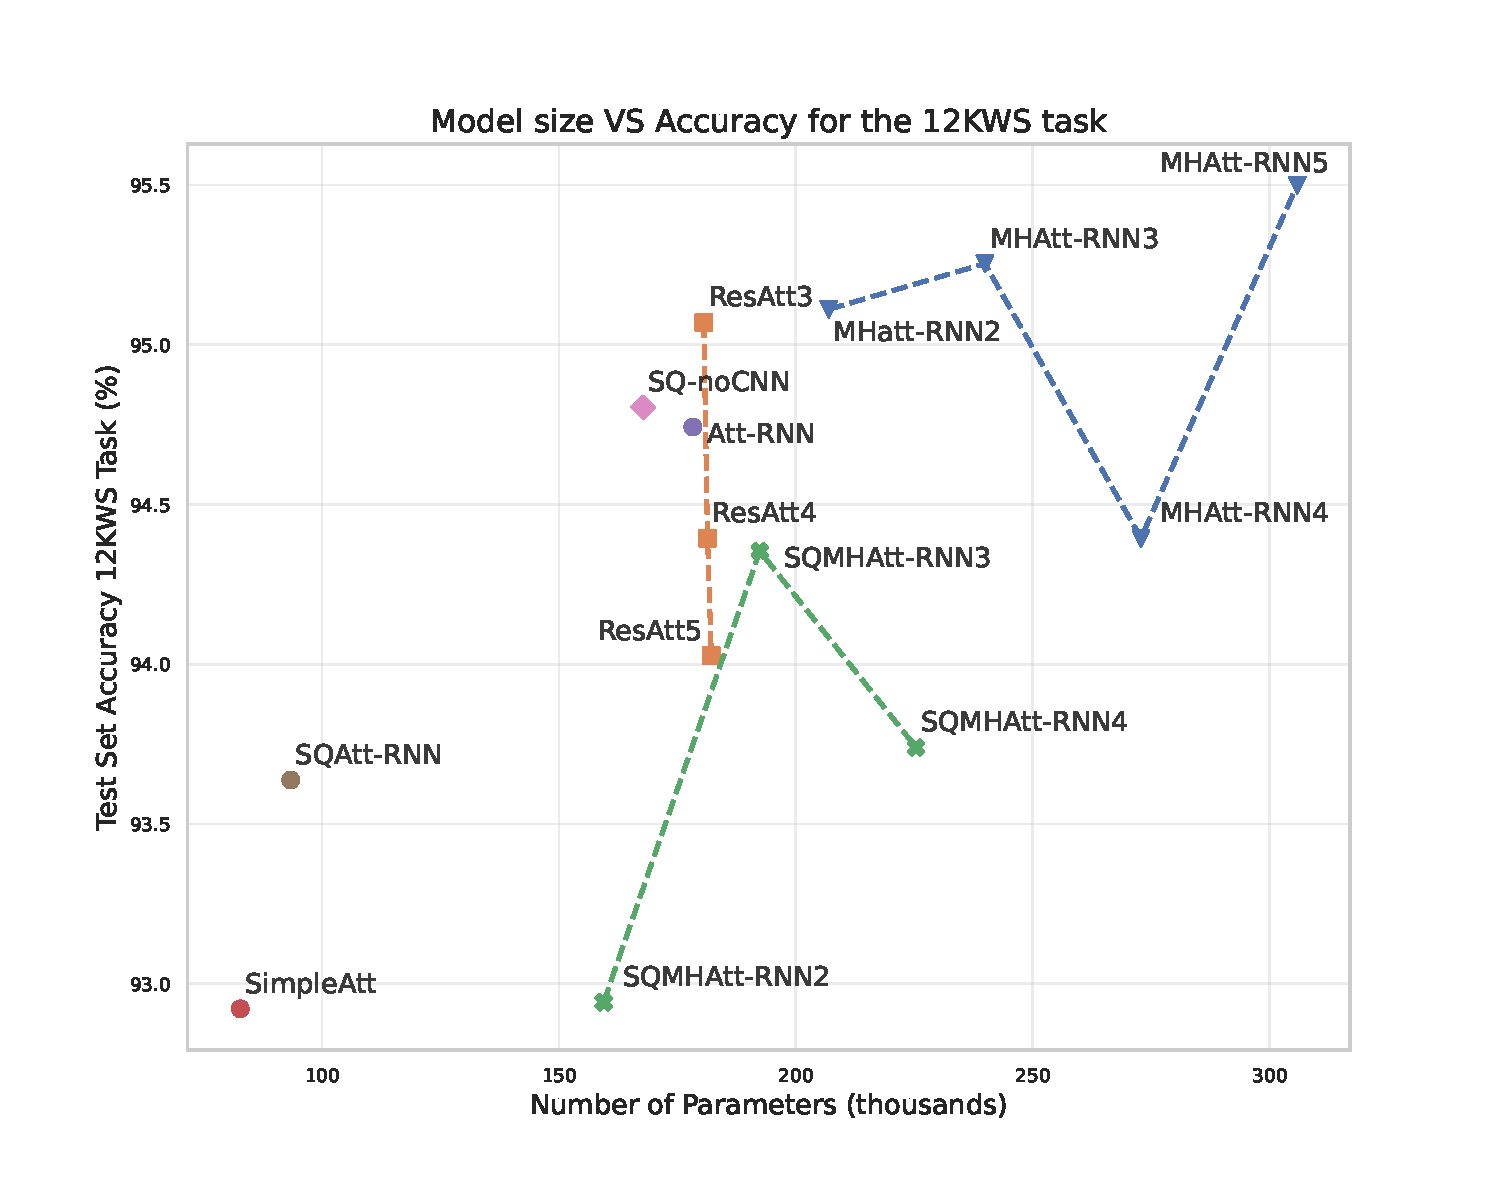
\includegraphics[width=\linewidth]{imgs/size_vs_accuracy12.pdf}
		\caption{A subfigure}
		\label{fig:sub1}
	\end{subfigure}%
	\begin{subfigure}{.5\textwidth}
		\centering
		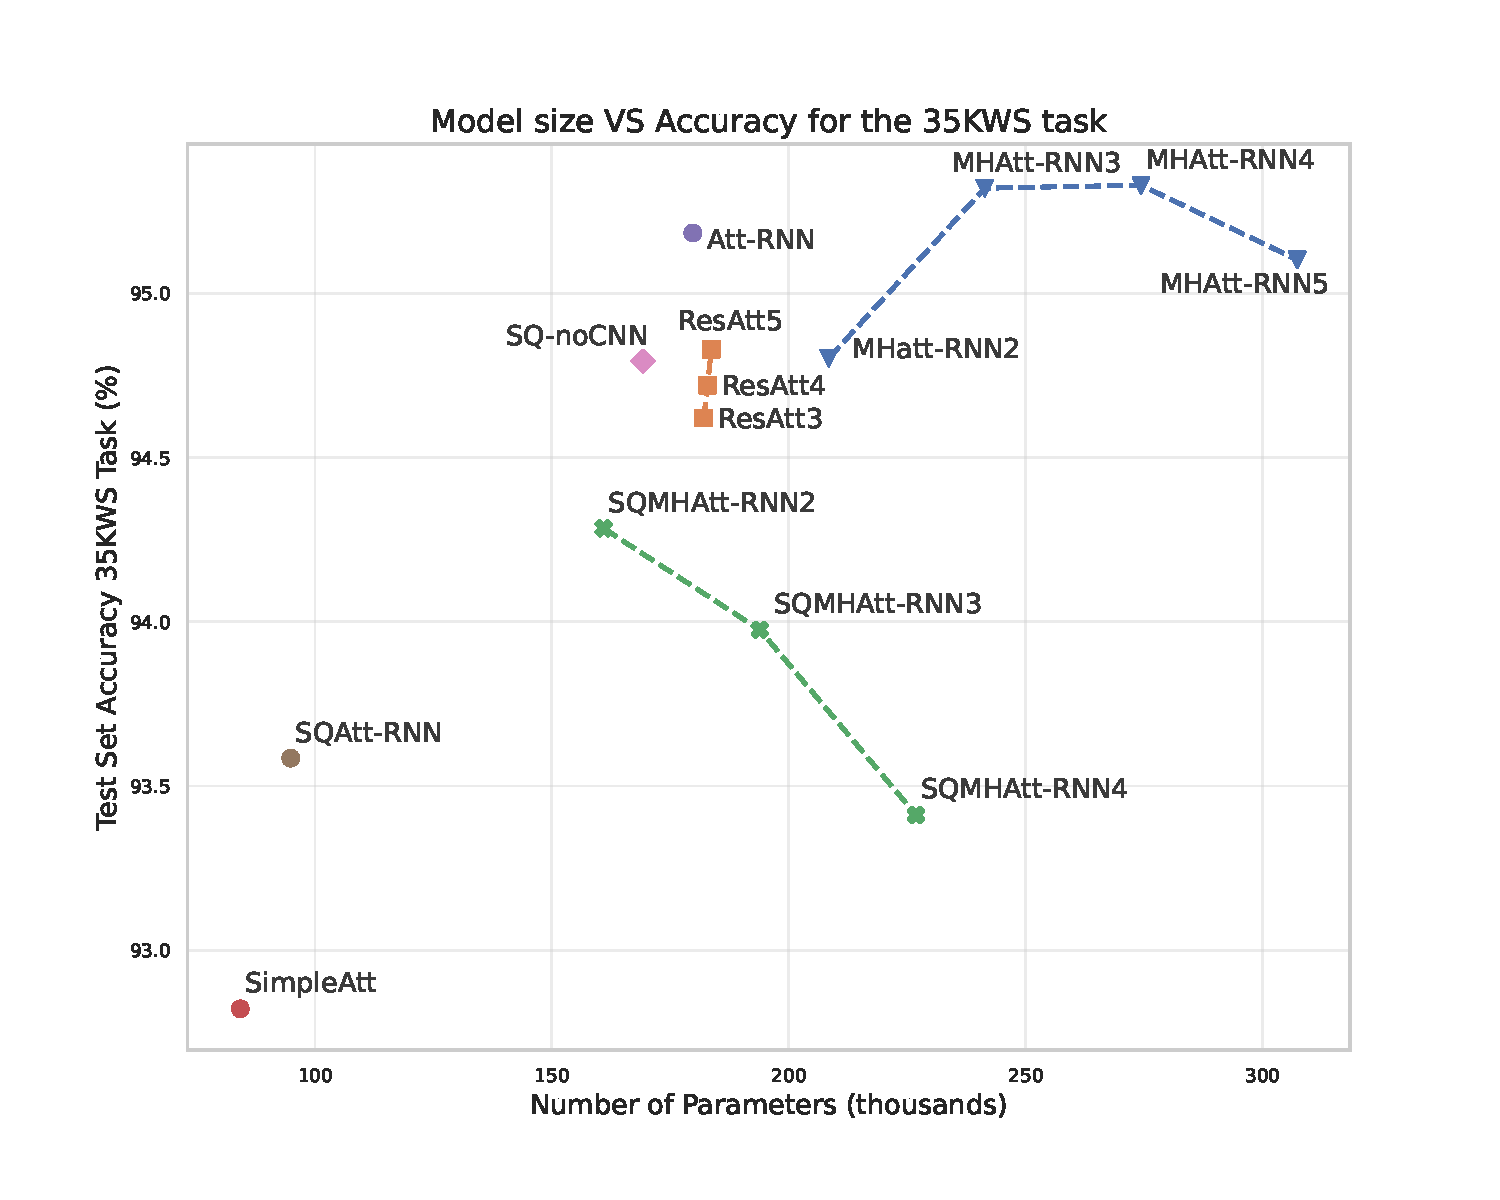
\includegraphics[width=\linewidth]{imgs/size_vs_accuracy35.pdf}
		\caption{A subfigure}
		\label{fig:sub2}
	\end{subfigure}
	\caption{A figure with two subfigures}
	\label{fig:accs_vs_parameters}
\end{figure*}

\begin{table}

	\caption{Table with results}

\begin{tabular}{lccc}	
	\hline 
	Model & Param. & Acc. 12kw & Acc. 35kw \\
	\hline \hline
	
	\rule{0pt}{3ex}SimpleAtt & $84 \mathrm{~K}$ & $92.9 \%$ & $92.8 \%$ \\
	Att-RNN & $180 \mathrm{~K}$& $94.7 \%$& $95.2 \%$ \\
	\hline 
	\rule{0pt}{3ex}SQAtt-RNN & $169 \mathrm{~K}$  & $94.9 \%$& $94.6 \%$ \\
	SQAtt-noCNN & $169 \mathrm{~K}$ & $94.8 \%$& $94.8 \%$ \\
	\hline \rule{0pt}{3ex}MHAtt-RNN2 & $208 \mathrm{~K}$ & $95.1 \%$& $94.8 \%$ \\
	MHAtt-RNN3 & $241 \mathrm{~K}$ & $95.2 \%$ & $95.3 \%$\\
	MHAtt-RNN4 & $274 \mathrm{~K}$ & $ 94.4\%$& $95.3 \%$ \\
	MHAtt-RNN5 & $307 \mathrm{~K}$ & $ 95.5\%$& $95.1 \%$ \\
	\hline \rule{0pt}{3ex}SQMHAtt-RNN2 &$235 \mathrm{~K}$ & $95.3 \%$& $\mathbf{95.4} \%$ \\
	SQMHAtt-RNN3 &$268 \mathrm{~K}$ & $95.4 \%$& $94.4 \%$ \\
	SQMHAtt-RNN4& $301 \mathrm{~K}$ & $94.7 \%$& $94.3 \%$ \\
	SQMHAtt-RNN5& $334 \mathrm{~K}$ & $\mathbf{95.7 \%}$& $95.0 \%$ \\
	\hline \rule{0pt}{3ex}Res-AttRNN3 &$182 \mathrm{~K}$ & $95.1\%$& $94.6 \%$ \\
	Res-AttRNN4& $183 \mathrm{~K}$ & $94.4 \%$& $94.7 \%$ \\
	Res-AttRNN5& $184 \mathrm{~K}$ & $94.0\%$& $94.8 \%$ \\
	\hline
	
	\label{table:results}
\end{tabular}
\end{table}
\subsection{Attention Plots}
As already mentioned, a really convenient feature of models based on attention is that it is easy to interpret them. Specifcally, we can plot the attention scores for our models to see which portions of the audio files were more important for the model in order to perform inference. In Figure \ref{fig:att_scores} we visualize log attention weights for Att-RNN and MHAtt-RNN3 models. 
\begin{figure}
	\centering
	\begin{tabular}{cc}
		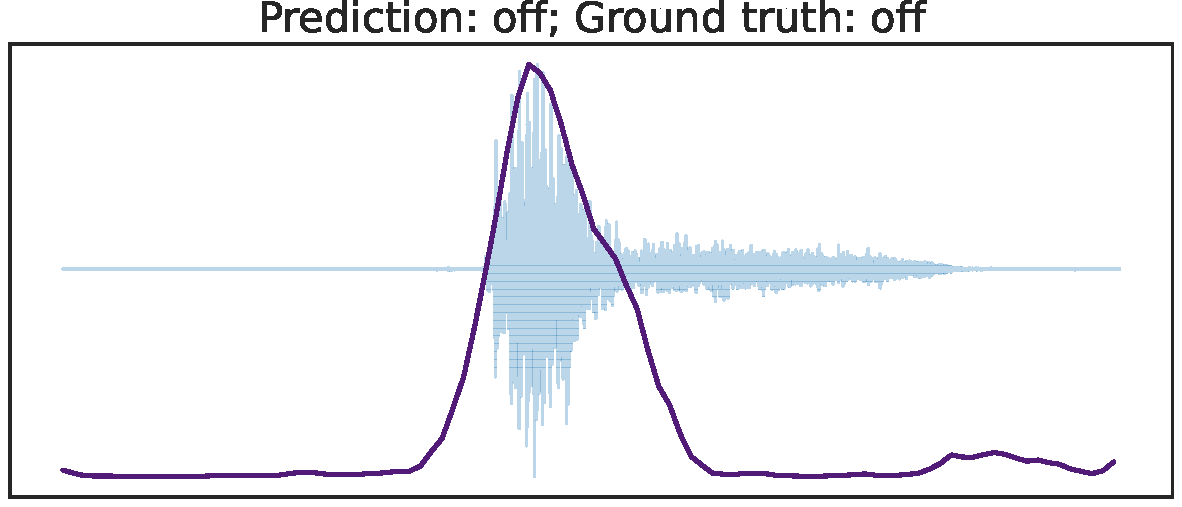
\includegraphics[width = 0.45\linewidth]{imgs/att_scores12_23_andreade.pdf} &
		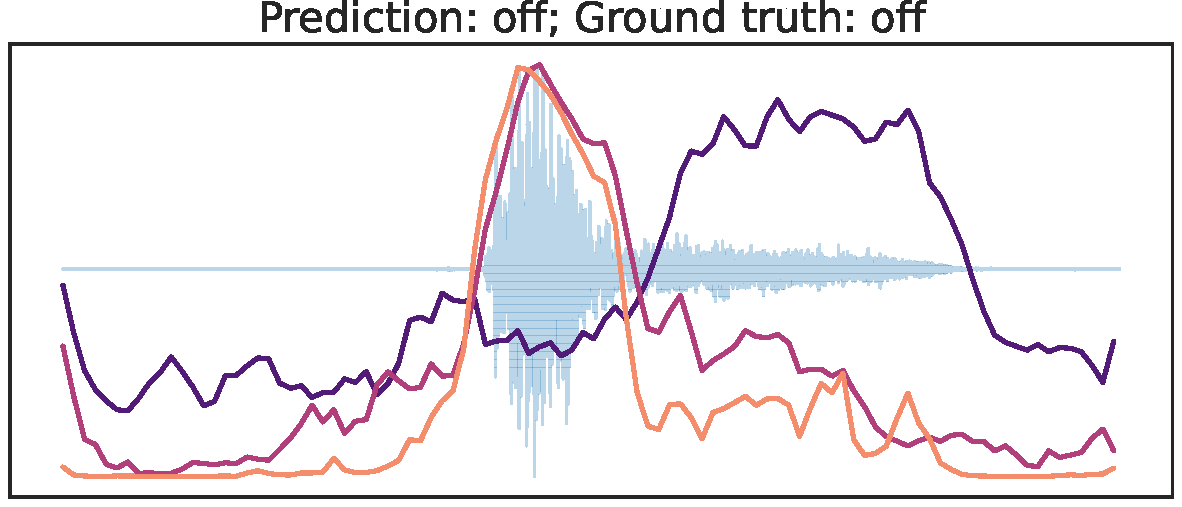
\includegraphics[width = 0.45\linewidth]{imgs/att_scores12_23.pdf}\\
		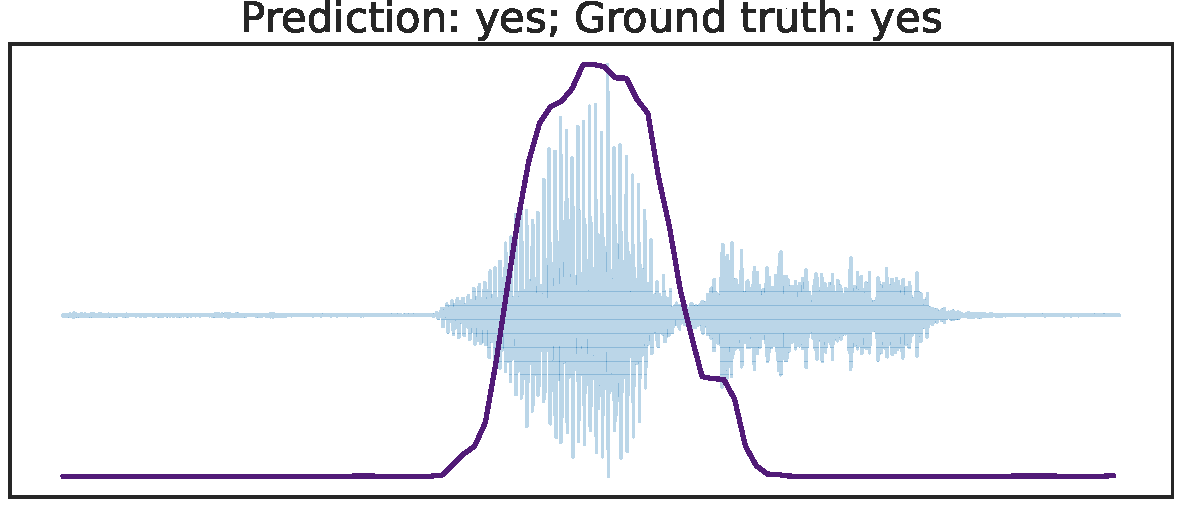
\includegraphics[width = 0.45\linewidth]{imgs/att_scores12_42_andreade.pdf} &
		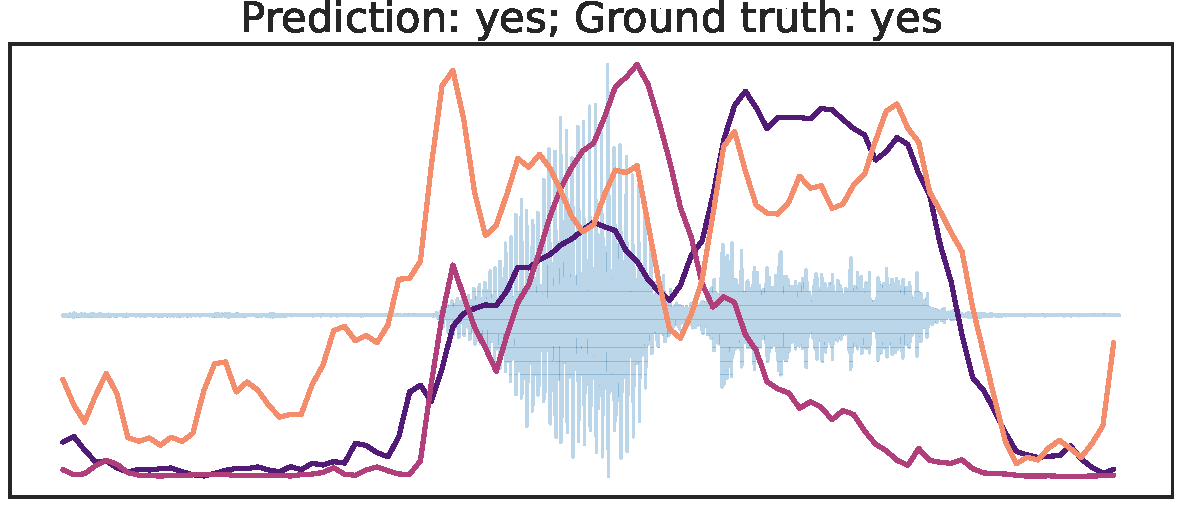
\includegraphics[width = 0.45\linewidth]{imgs/att_scores12_42.pdf}\\
		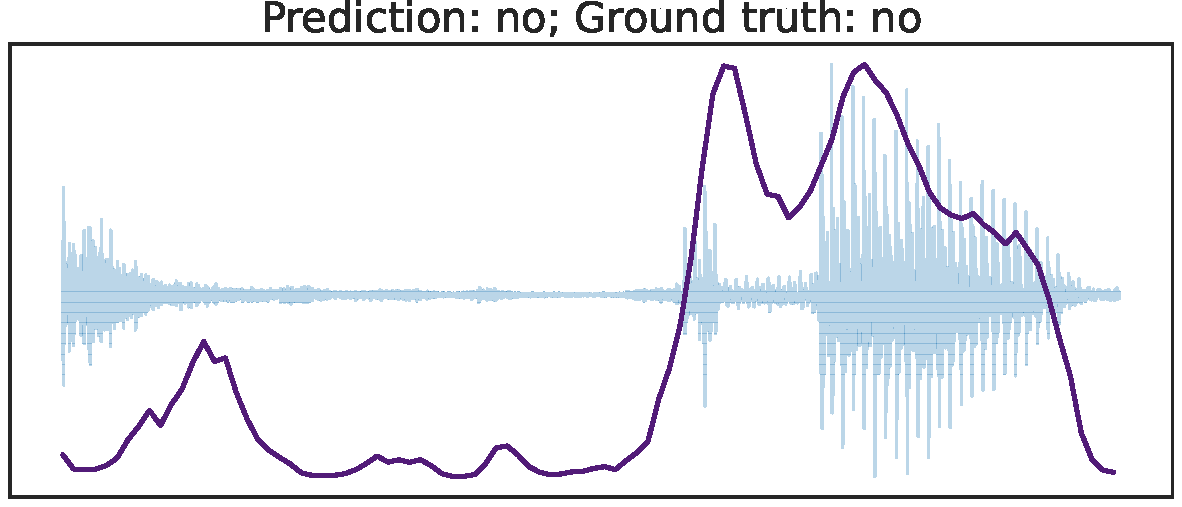
\includegraphics[width = 0.45\linewidth]{imgs/att_scores12_72_andreade.pdf} &
		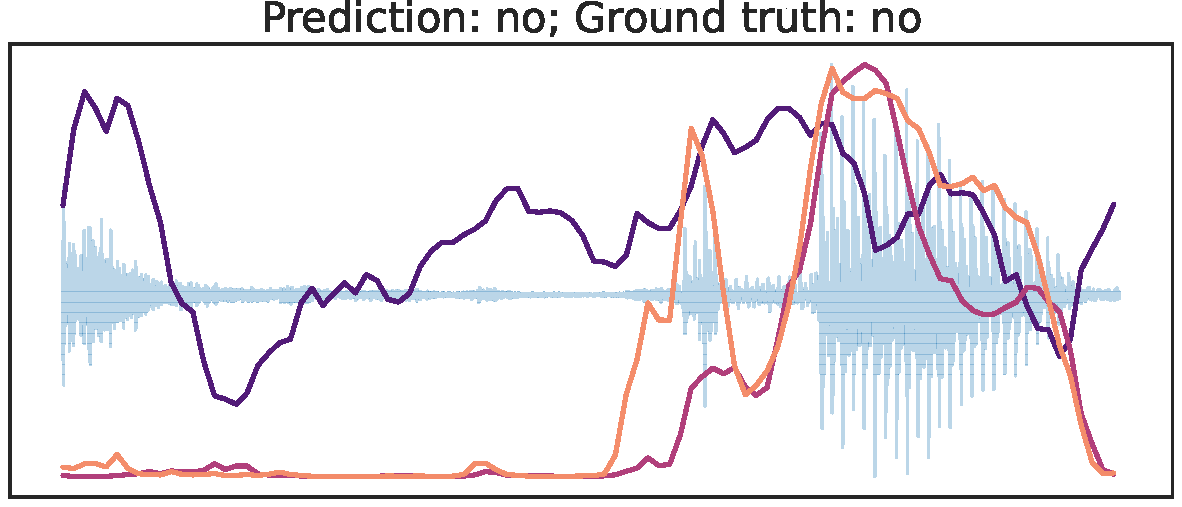
\includegraphics[width = 0.45\linewidth]{imgs/att_scores12_72.pdf}
	\end{tabular}
	\caption{Comparison between attention scores from  Att-RNN model (left) and MHAtt-RNN3 (right), on the words \textit{off}, \textit{yes} and \textit{no}. }
	\label{fig:att_scores}
\end{figure}
We can see that Att-RNN has only one head, so one set of attention scores per prediction is computed. MHAtt-RNN instead computes one set of attention weights per head: here we visualize the attention scores for each head. In these examples, we can see how each head learns to pay attention to different phonemes of the same word. In the first example, Att-RNN pays attention only to the first phoneme /\textipa{o}/, while MHAtt-RNN has two heads paying attention to /o/ and one paying attention to /f/. In the second example, a similar thing happens: Att-RNN pays attention just at the phoneme /\textipa{je}/ while MHAtt-RNN has different heads concentrating both on /\textipa{je}/ and /\textipa{s}/. The third example presents a noise at the beginning which is not part of the spoken word: Att-RNN has its attention drawn a bit, while two of three heads from MHAtt-RNN learn to completely ignore it.


